% sec_experiments_journal_p4.tex  (intervention analysis + failure modes)

\subsection{Concept Intervention Analysis}
\label{sec:intervention}

A key promise of concept bottleneck architectures is \emph{intervenability}:
a user can inspect a concept, judge it mis-estimated, and correct it
without retraining the full network.
For accident anticipation this matters because many practical errors are
tied to \emph{under-activation} of an intuitively correct risk concept.
We provide two levels of evidence.

\paragraph{Stored-trajectory intervention.}
For a false-negative or borderline DAD case, we identify one concept whose
activation is visually inconsistent with the scene semantics (e.g., a
cut-in vehicle is clearly present but the concept response is weak).
We increase that concept's activation in the pre-crash window and
compare the original and edited alert trajectories.

\begin{figure*}[t]
  \centering
  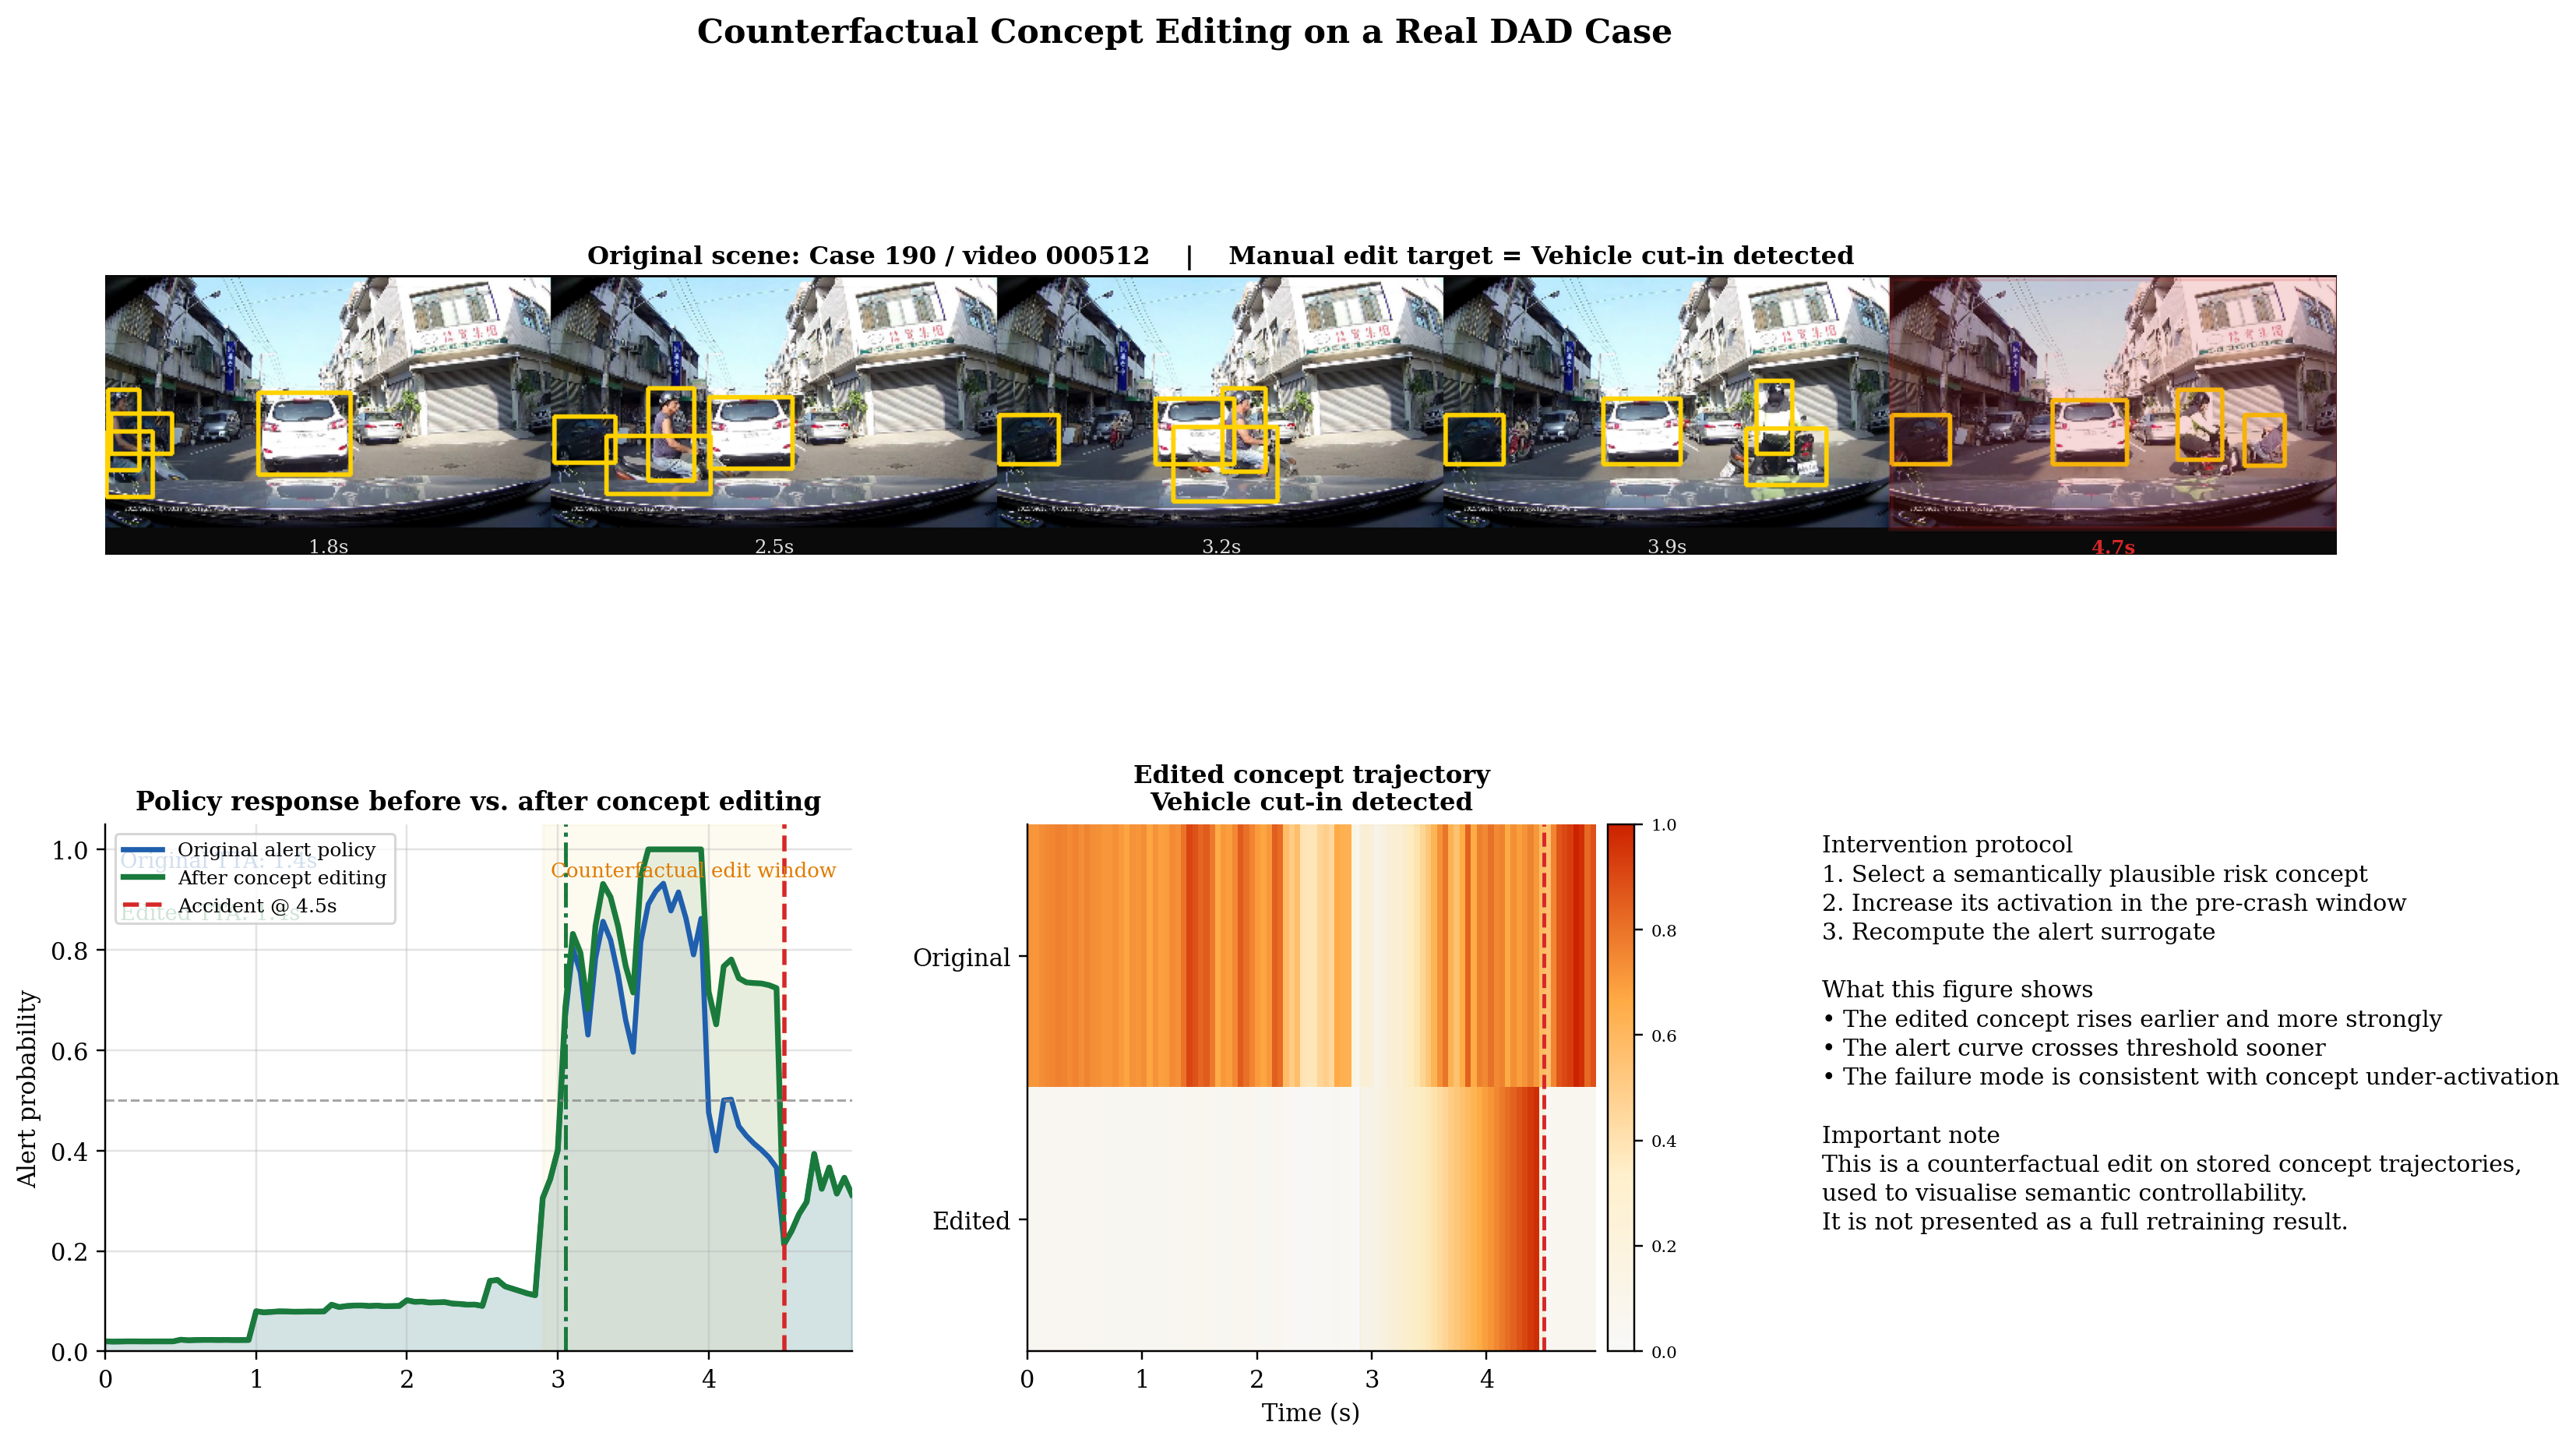
\includegraphics[width=\textwidth]{../figures/insight_fig_appendix_intervention.png}
  \caption{\textbf{Counterfactual concept editing on a real DAD case.}
  We increase the activation of concept \texttt{Vehicle cut-in detected}
  in the pre-crash window. The edited alert curve crosses the threshold
  earlier than the original, demonstrating that \method{} exposes a
  semantically meaningful control surface.
  This is a counterfactual edit on stored concept trajectories, not
  a full retraining result.}
  \label{fig:intervention}
\end{figure*}

Figure~\ref{fig:intervention} shows that a semantically valid positive edit
moves the alert earlier---exactly the expected behaviour of a
concept-conditioned timing model. The timing decision is responsive to
semantically relevant risk evidence rather than locked inside an opaque
latent space.

\paragraph{Backbone-level re-run.}
To go beyond cached curves, we load the available v4 DAD checkpoint,
apply a concept-channel edit, and re-run the downstream prediction branch.
This produces a more faithful intervention path through the model backbone.

\begin{figure*}[t]
  \centering
  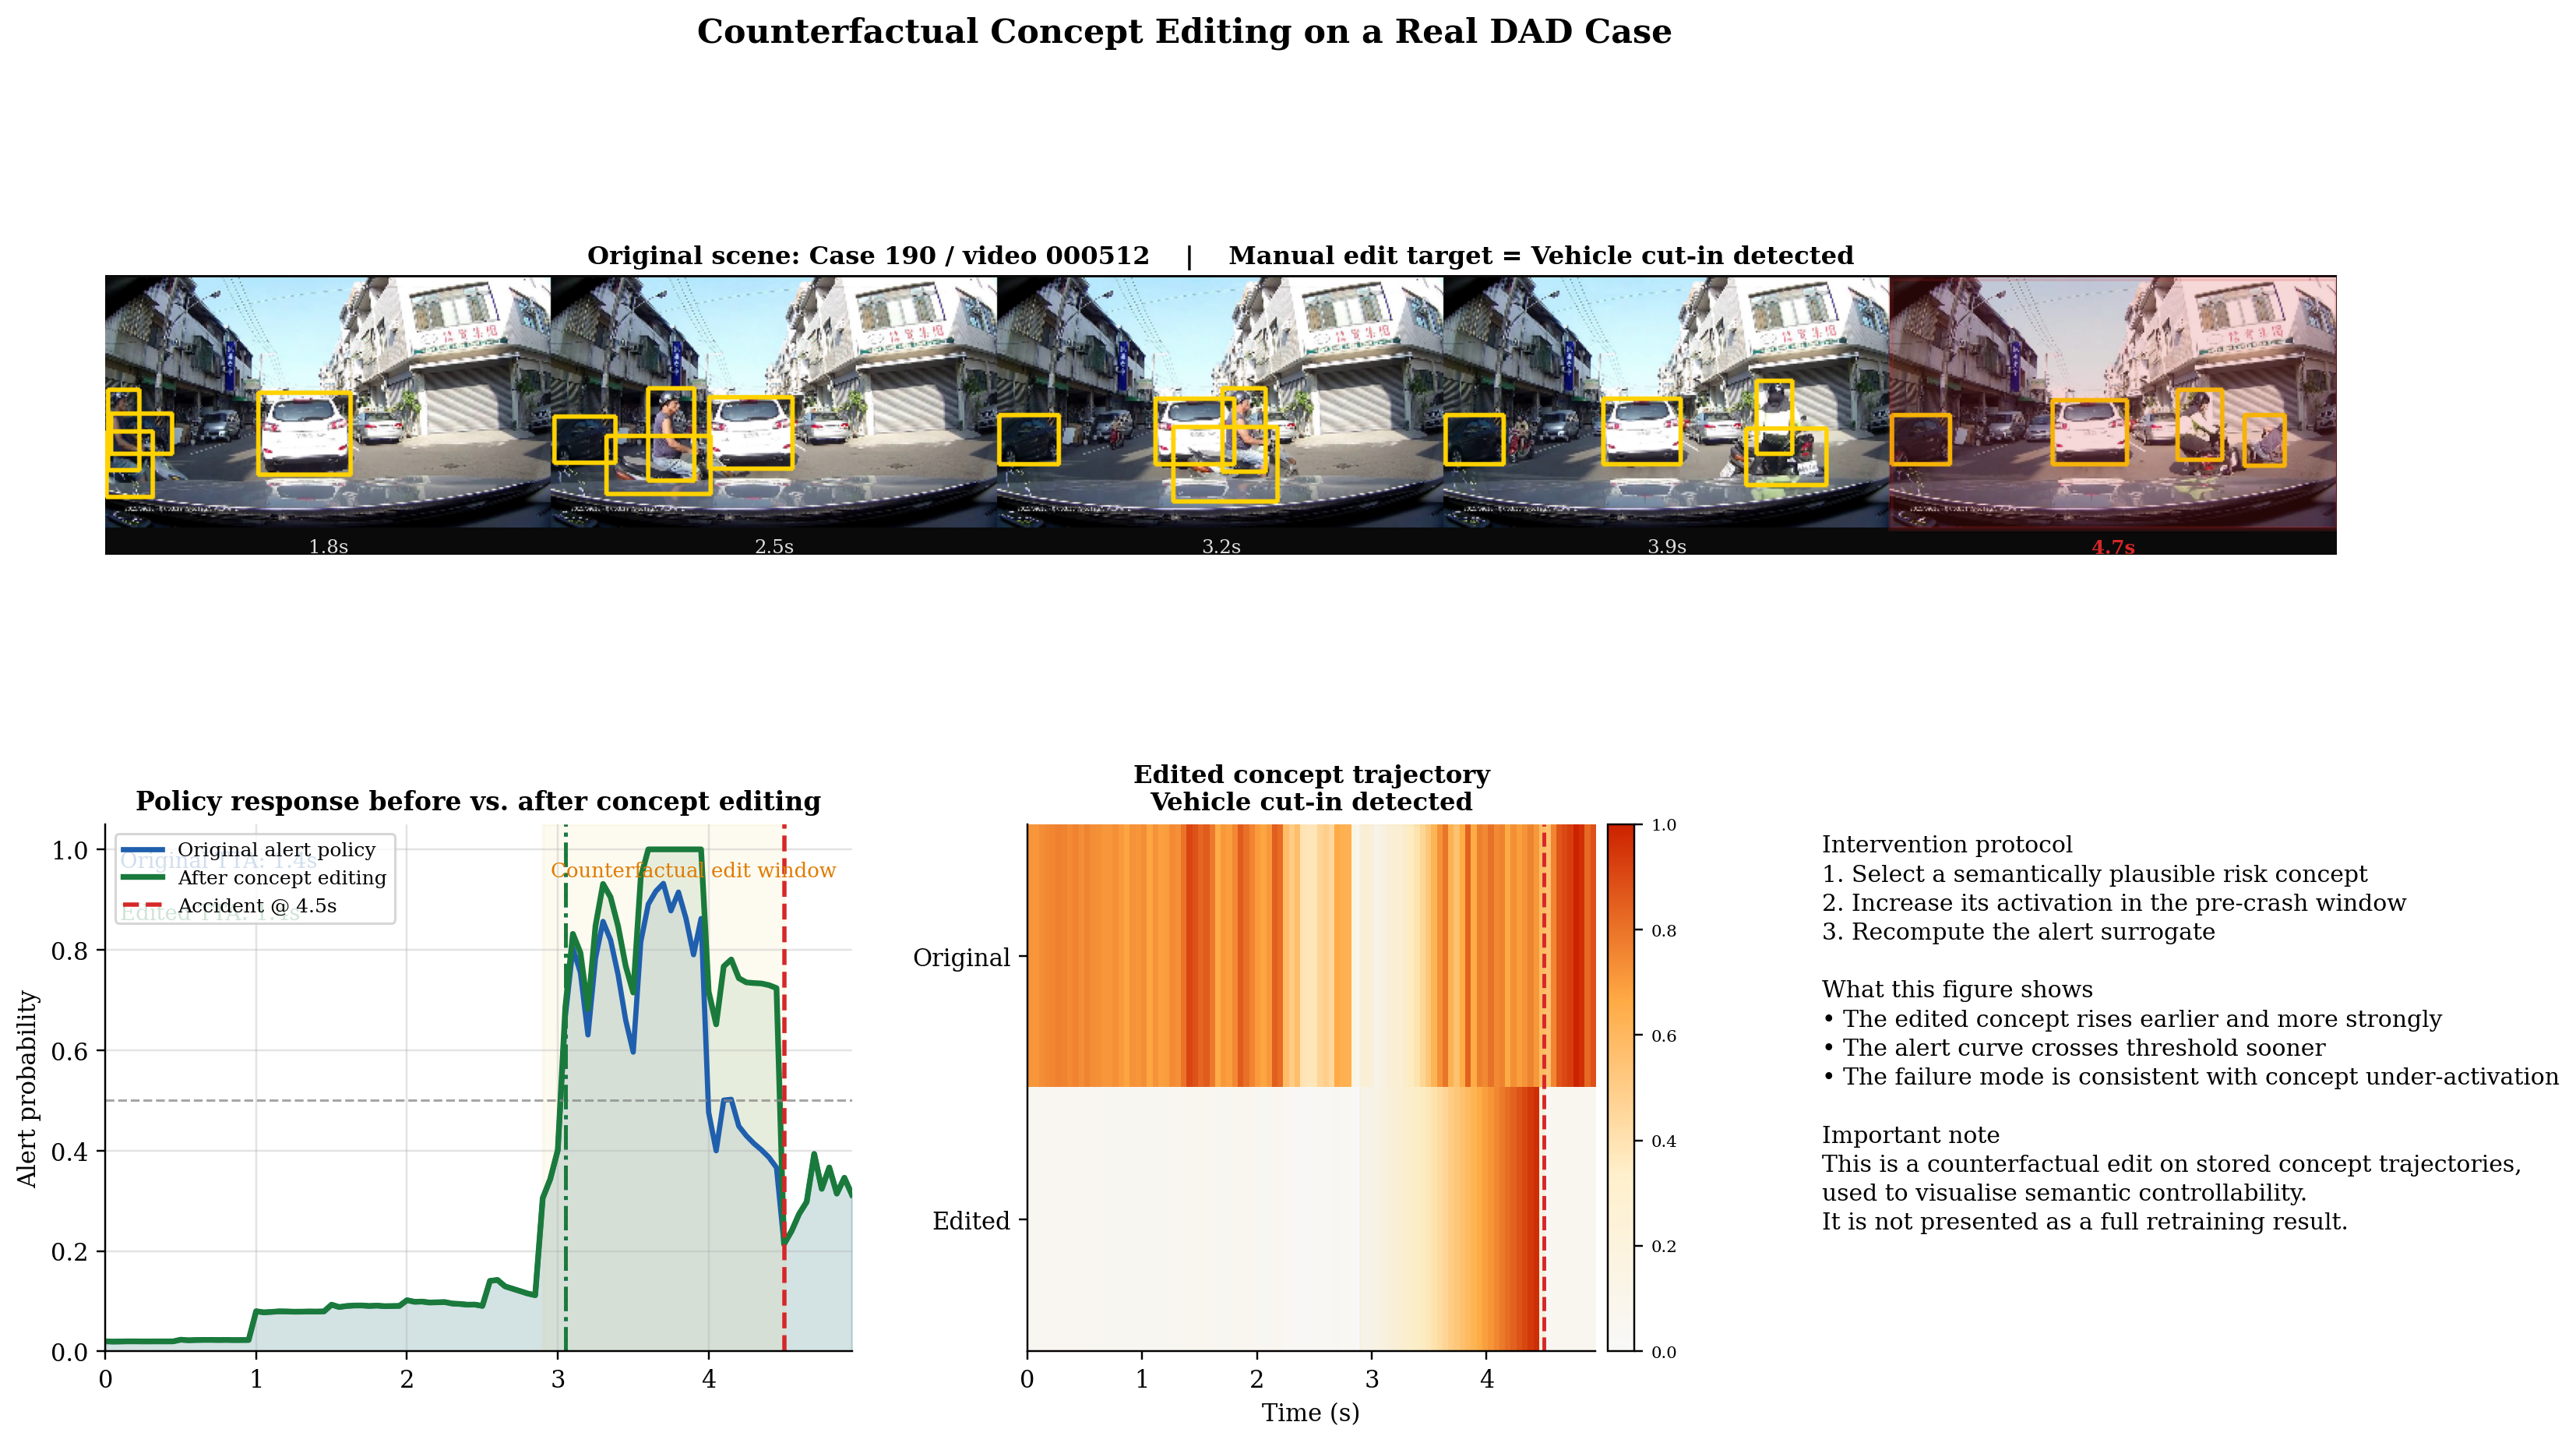
\includegraphics[width=\textwidth]{../figures/insight_fig_appendix_intervention_v4_backbone.png}
  \caption{\textbf{Backbone-level intervention re-run (v4 DAD checkpoint).}
  Concept edit is passed back through the loaded backbone rather than
  only modifying a stored output curve. The available checkpoint does not
  contain the final Actor--Critic head weights; the result should be
  read as a backbone-level re-run, not a full policy-level intervention.}
  \label{fig:intervention_v4}
\end{figure*}

The backbone-level re-run confirms that concept edits propagate through
the loaded model and change downstream prediction behaviour.
However, an automatic search across positive DAD test cases revealed
that large timing shifts are not uniformly common under this incomplete
checkpoint line---the most frequent outcome is a modest amplitude
increase with little threshold-crossing change.
We view this as an important boundary condition: concept-conditioned
controllability is real but not uniformly strong under all checkpoints.
We therefore scope the v4 result as a backbone-level intervention
demonstration rather than a full policy-level causal robustness claim.

\begin{table}[t]
\caption{\textbf{Structured summary of intervention evidence.}
Columns describe what each evidence source does and does not establish.}
\label{tab:intervention_summary}
\centering\small
\begin{tabular}{p{0.27\linewidth}p{0.32\linewidth}p{0.30\linewidth}}
\toprule
Evidence & Supports & Does \emph{not} imply\\
\midrule
Stored-trajectory edit
  & Concept edits shift alert earlier in a semantically consistent direction
  & Not a full model re-run; not a policy-level causal test\\
Backbone-level v4 re-run
  & Edits propagate through the loaded backbone and alter prediction
  & Does not establish uniform timing controllability across DAD\\
Automatic v4 search
  & Result is not cherry-picked; broader scan conducted
  & Large timing gains not common under incomplete checkpoint line\\
Case bank screening
  & WHY/WHEN evidence visible across multiple scenes
  & Not every scene yields equally legible frame-level explanations\\
\bottomrule
\end{tabular}
\end{table}

\begin{figure*}[t]
  \centering
  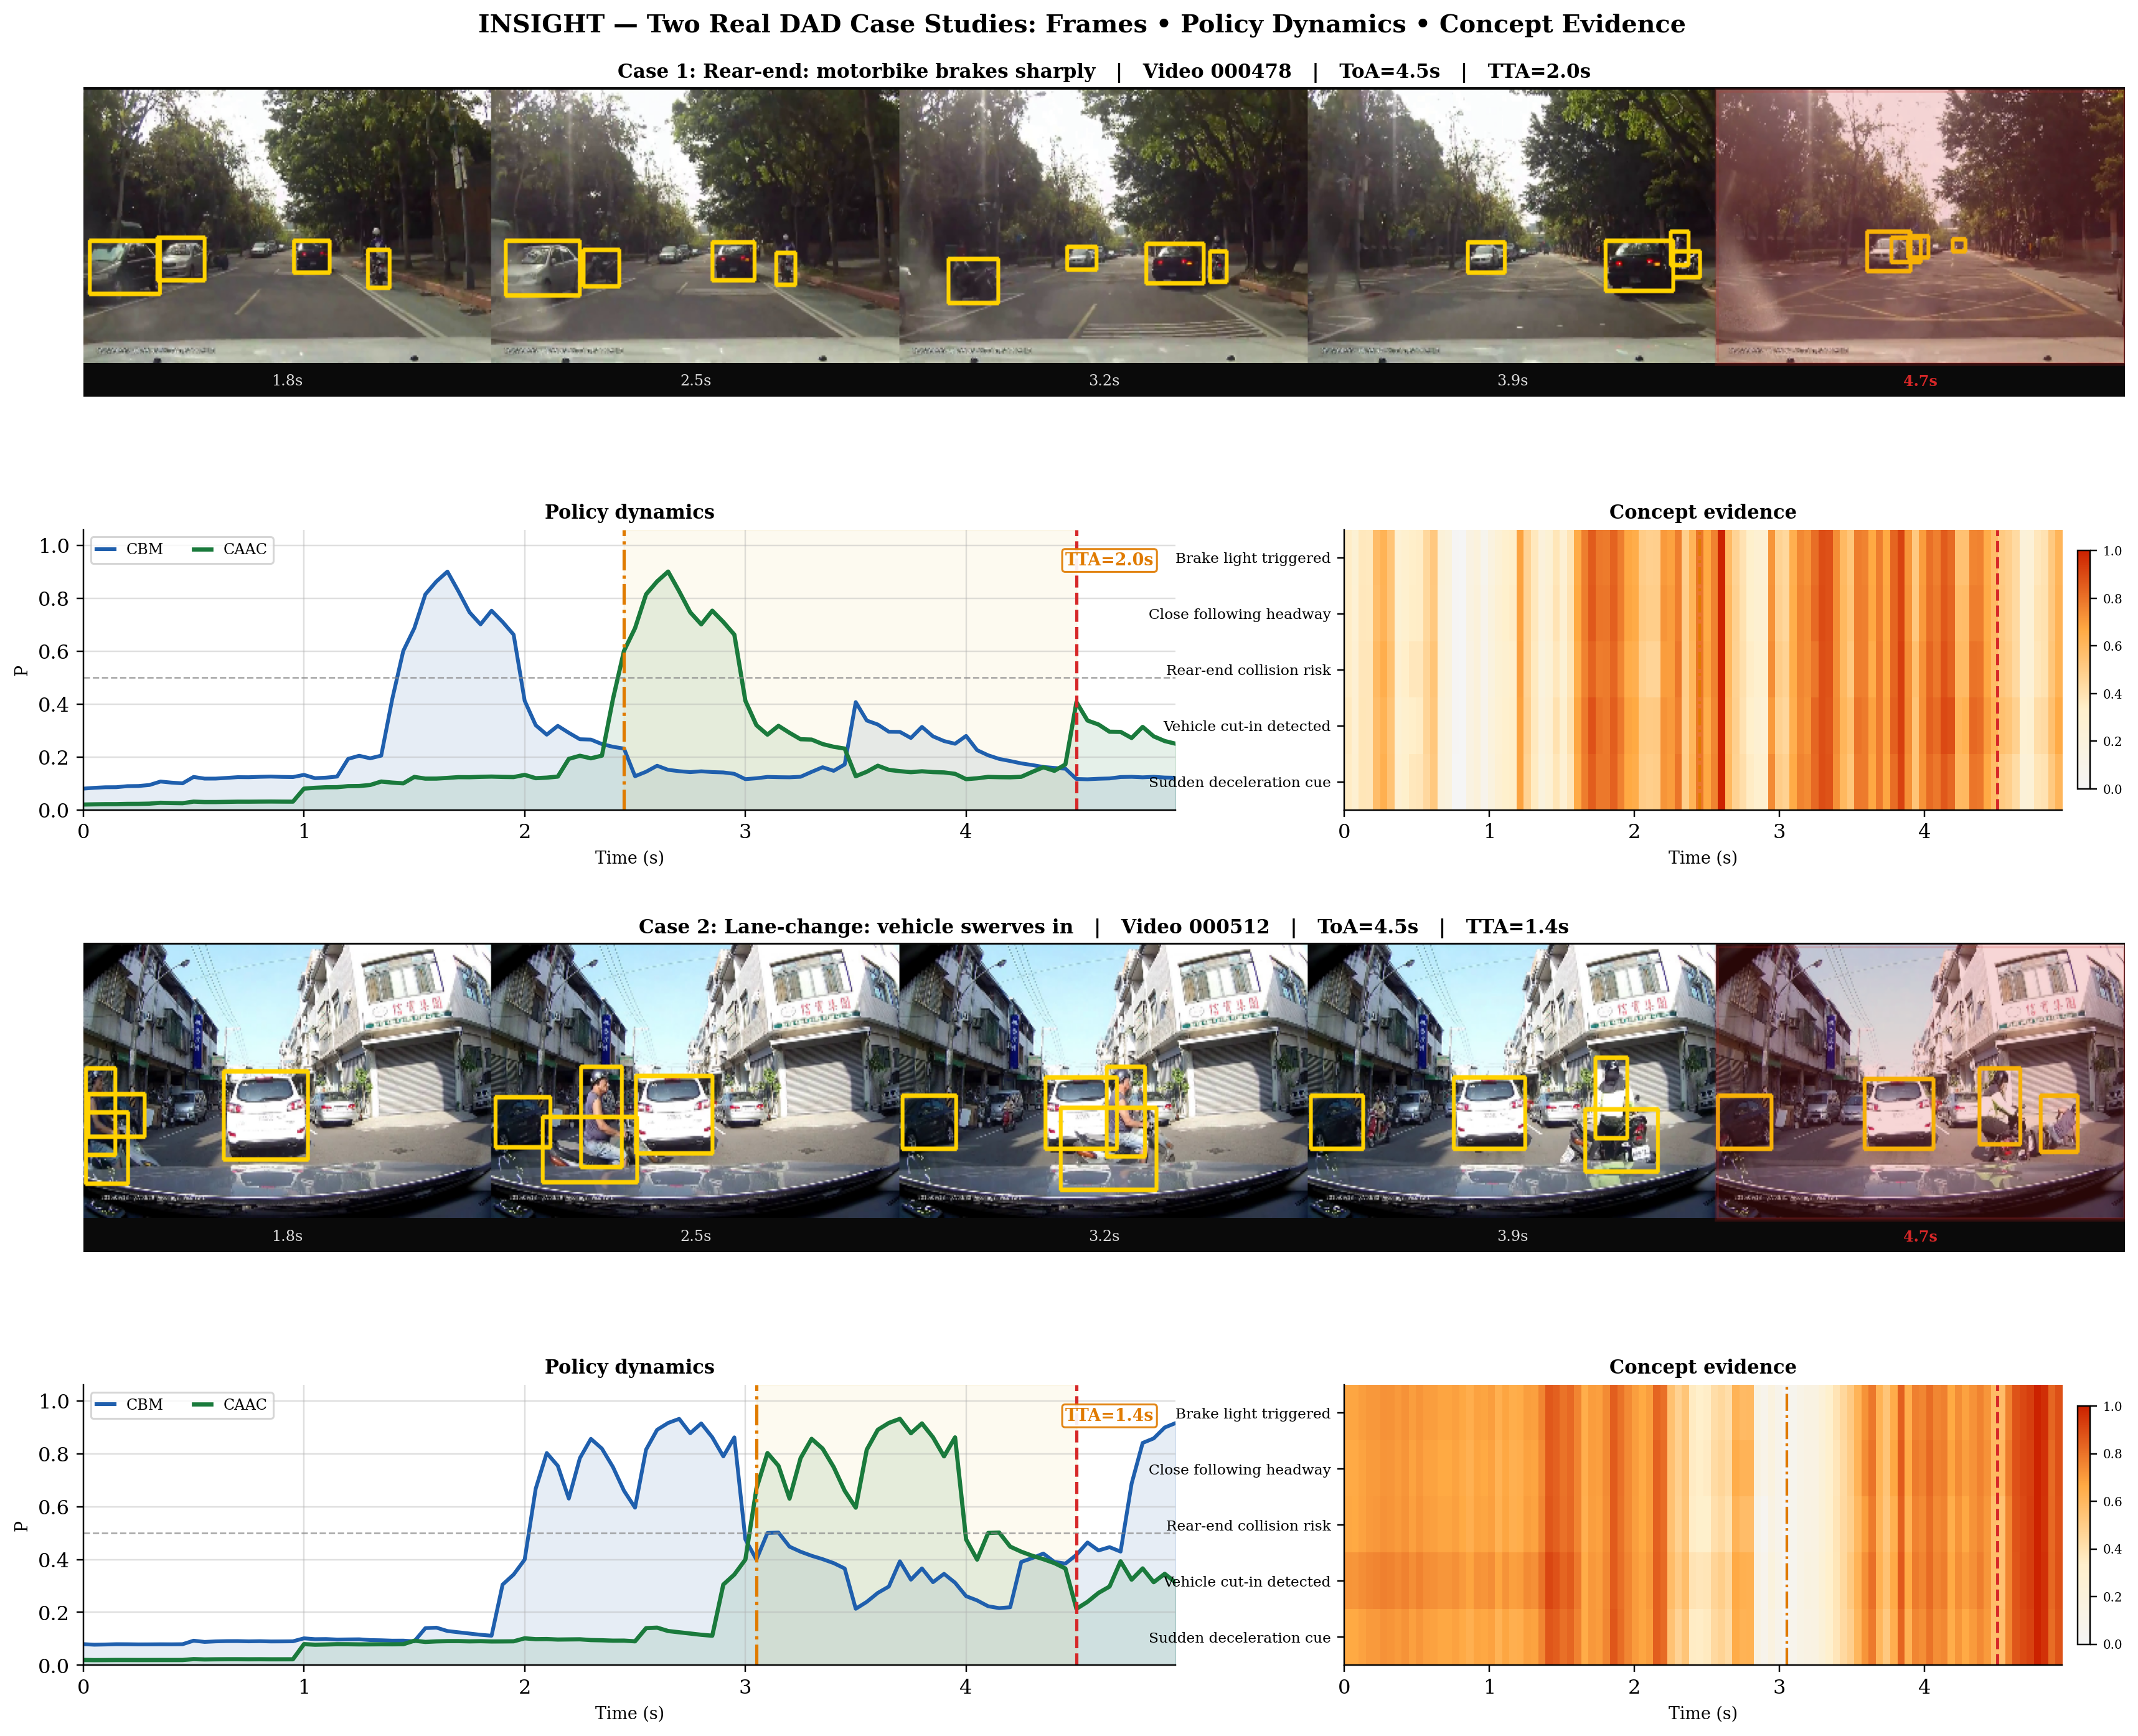
\includegraphics[width=0.98\textwidth]{../figures/insight_fig_appendix_v4_casebank_selected.png}
  \caption{\textbf{Selected v4 DAD cases ranked by prediction-branch behaviour.}
  A shortlist covering an earlier-warning case, borderline cases, and a
  low-visibility example. Read as a prediction-level qualitative bank
  for concept-pattern diversity and timing contrast, not a policy-level
  alert benchmark.}
  \label{fig:v4_casebank}
\end{figure*}

\subsection{Failure Modes and Robustness Considerations}
\label{sec:failure}

\paragraph{Low-visibility conditions.}
Night-time and poor-weather scenes weaken ROI features and reduce concept
reliability, especially for fine-grained cues (brake lights, lane markings).
The typical failure mode is concept under-activation rather than an
incorrect timing policy.

\paragraph{Crowded scenes.}
When many agents co-occur, object-focused aggregation must compress rich
interaction structure into a fixed hidden state, potentially diluting the
most critical risk agent. Explicit risk-agent selection is a natural
journal-version extension.

\paragraph{Concept vocabulary coverage.}
With 837 concepts, rare corner cases may fall outside the vocabulary.
Hierarchical or adaptive concept sets that retain auditing benefits
while improving long-tail coverage are a promising direction.

\paragraph{Why A3D and DAD behave differently.}
A3D hazards develop progressively, so early concept growth is especially
valuable. DAD margins are tighter and scenes more cluttered---a harder
benchmark that stress-tests concept reliability. This explains why DAD
yields smaller but still meaningful gains in the interpretable tier.
